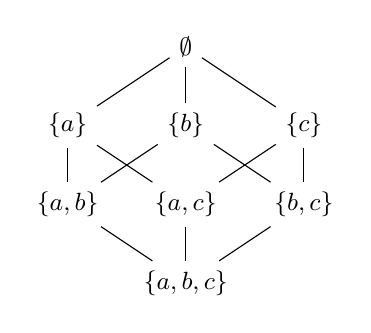
\begin{tikzpicture}[every node/.style={font=\small}]
  % Level 0
  \node (empty) at (0,0) {$\emptyset$};
  % Level 1
  \node (a) at (-1.5,-1) {$\{a\}$};
  \node (b) at (0,-1) {$\{b\}$};
  \node (c) at (1.5,-1) {$\{c\}$};
  % Level 2
  \node (ab) at (-1.5,-2) {$\{a,b\}$};
  \node (ac) at (0,-2) {$\{a,c\}$};
  \node (bc) at (1.5,-2) {$\{b,c\}$};
  % Level 3
  \node (abc) at (0,-3) {$\{a,b,c\}$};
  % Edges
  \foreach \x/\y in {
    empty/a,empty/b,empty/c,
    a/ab,a/ac,
    b/ab,b/bc,
    c/ac,c/bc,
    ab/abc,ac/abc,bc/abc}
    \draw (\x)--(\y);
\end{tikzpicture}

%%% Local Variables:
%%% mode: latex
%%% TeX-master: "../main"
%%% End:
